\documentclass[a4paper,12pt]{article}
\usepackage[latin1]{inputenc}
\usepackage[spanish]{babel}
\usepackage{bm}
\usepackage{graphicx}
\usepackage{amsmath}
\setlength{\textheight}{235mm}
\setlength{\textwidth}{168mm}
\setlength{\oddsidemargin}{0pt}
\pagestyle{empty}
\begin{document}
\mbox{}\vspace*{-45mm}

{\centering
{\small\sc Escuela T�cnica Superior de Ingenieros de Caminos, Canales y
Puertos (Madrid)}\\*[4mm]
{\Large\bf M�todo de los Elementos Finitos (Curso 22-23). Examen extraordinario (26/01/2023)}\\*[4mm]
Ejercicio 1: Estructuras de barras articuladas \\*[4mm]
}

\vspace{3mm}

%%%%%
\noindent

Se tiene la estructura de barras articuladas (viga Pratt) mostrada en la figura debajo. El m�dulo de elasticidad es $E= 210\,\mbox{GPa}$. El �rea de la secci�n transversal es $A=20\cdot 10^3\,\mbox{mm}^2$. 

Las dimensiones, condiciones de contorno de la estructura y cargas aplicadas se indican en la figura. 

Se pide hacer un modelo de elementos finitos que permita conocer la respuesta mec�nica de la estructura y contestar el cuestionario. 

\begin{center}
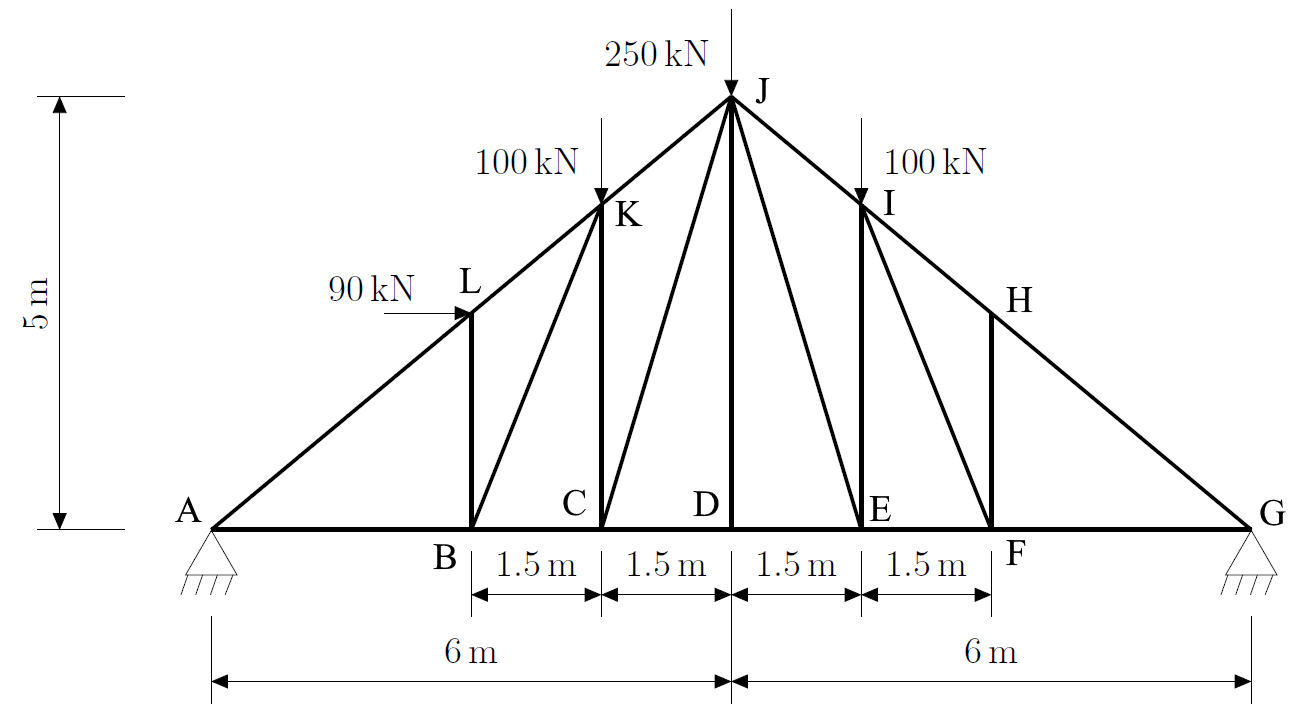
\includegraphics[width=0.9\textwidth]{figura_pratt}
\end{center}
\end{document}
